\documentclass{standalone}
\usepackage{tikz} % Import the tikz package
\usetikzlibrary{automata} % Import library for drawing automata
\usetikzlibrary{positioning} % ...positioning nodes
\usetikzlibrary{arrows} % ...customizing arrows
\tikzset{node distance=2.5cm,
    every state/.style={
        semithick,
        fill=gray!10},
    initial text={},
    double distance=2pt,
    every edge/.style={
        draw,
        ->,>=stealth',
        auto,
        semithick}}
\let\epsilon\varepsilon
\begin{document}
    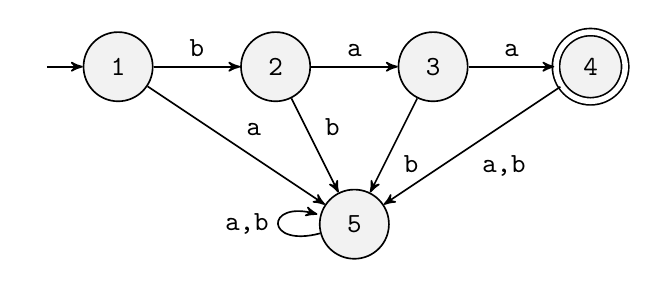
\begin{tikzpicture}
        \node[state, initial] (1) at (0,0) {\tt 1};
        \node[state] (2) at (2,0) {\tt 2};
        \node[state] (3) at (4,0) {\tt 3};
        \node[state,accepting] (4) at (6,0) {\tt 4};
        \node[state] (5) at (3,-2) {\tt 5};
        
        \draw (1) edge[] node {\tt b} (2);
        \draw (1) edge[] node {\tt a} (5);

        \draw (2) edge[] node {\tt a} (3);
        \draw (2) edge[] node {\tt b} (5);

        \draw (3) edge[] node {\tt a} (4);
        \draw (3) edge[] node {\tt b} (5);

        \draw (4) edge[] node {\tt a,b} (5);

        \draw (5) edge[loop left] node {\tt a,b} (5);
    \end{tikzpicture}
\end{document}